\de{ĐỀ THI HỌC KỲ I NĂM HỌC 2022-2023}{Trường THPT Võ Nguyên Giáp - Quảng Nam}

\begin{center}
	\textbf{PHẦN 1 - TRẮC NGHIỆM}
\end{center}

\setcounter{ex}{0}\setcounter{bt}{0}
\Opensolutionfile{ans}[ans/ans-0-HK1-1-VoNguyenGiap-2223]

\subsection*{I. PHẦN TRẮC NGHIỆM}

%Câu 1
\begin{ex}%[0D1K3-3]%[Dự án đề kiểm tra HKI NH22-23-VU Ngoc Hao]%[VoNguyenGiap-QuangNam]
	Lớp học có $7$ học sinh giỏi Toán, $5$ học sinh giỏi Lý, $6$ học sinh giỏi Hóa, $3$ học sinh giỏi cả Toán và Lý, $4$ học sinh giỏi cả Toán và Hóa, $2$ học sinh giỏi cả Lý và Hóa, $1$ học sinh giỏi cả ba môn Toán, Lý, Hóa. Số học sinh giỏi ít nhất một môn của lớp là
	\choice
	{$20$}
	{$28$}
	{$18$}
	{\True $10$}
	\loigiai{
		Gọi $A$ là tập hợp các học sinh giỏi Toán.\\
		Gọi $B$ là tập hợp các học sinh giỏi Lý.\\
		Gọi $C$ là tập hợp các học sinh giỏi Hóa.\\
		Theo đề bài, ta có $n(A)=7$, $n(B)=5$, $n(C)=6$, $n\left(A\cap B\right)=3$, $n\left(B\cap C\right)=4$, $n\left(C\cap A\right)=2$, $n\left(A\cap B\cap  C\right)=1$.\\
		Khi đó số học sinh giỏi ít nhất 1 môn trong lớp là
		\begin{eqnarray*}
		n\left(A\cup B\cup C\right) 
		&=& n(A) + n(B) + n(C) - n(A\cap B) - n(B\cap C) - n(C\cap A) + n(A\cap B\cap C)\\
		&=& 7 + 5 +6 -3 -4 - 2 +1\\
		&=& 10.
		\end{eqnarray*}
	}
\end{ex}

%Câu 2
\begin{ex}%[0H3Y1-3]%[Dự án đề kiểm tra HKI NH22-23-VU Ngoc Hao]%[VoNguyenGiap-QuangNam]
	Trong hệ trục $Oxy$ cho các véc-tơ $\overrightarrow{u}=5\overrightarrow{i} - 4\overrightarrow{j}$. Tọa độ của véc-tơ $\overrightarrow{u}$ được viết là
	\choice
	{$\overrightarrow{u}=(5;4)$}
	{$\overrightarrow{u}=(4;5)$}
	{$\overrightarrow{u}=(-4;5)$}
	{\True $\overrightarrow{u}=(5;-4)$}
	\loigiai{
		Ta có $\overrightarrow{u} = 5\overrightarrow{i} -4\overrightarrow{j} \Rightarrow \overrightarrow{u} = (5;-4)$.
	}
\end{ex}

%Câu 3
\begin{ex}%[0D2Y2-2]%[Dự án đề kiểm tra HKI NH22-23-VU Ngoc Hao]%[VoNguyenGiap-QuangNam]
	Điểm nào sau đây {\bf không} thuộc miền nghiệm của hệ bất phương trình $\heva{&x+y\geq 0\\&x+y -4 <0}$?
	\choice
	{$(1;1)$}
	{$(1;0)$}
	{$(-1;2)$}
	{\True $(3;4)$}
	\loigiai{
		Ta có với $x= 3$, $y=4$ thì $x+y-4 = 3 >0$.\\
		Suy ra điểm $(3;4)$ không thuộc miền nghiệm của hệ bất phương trình đã cho.
	}
\end{ex}

%Câu 4
\begin{ex}%[0H2Y4-1]%[Dự án đề kiểm tra HKI NH22-23-VU Ngoc Hao]%[VoNguyenGiap-QuangNam]
	Tích vô hướng của hai véc-tơ khác véc-tơ-không $\overrightarrow{u}$ và $\overrightarrow{v}$ là một số, được xác định bởi công thức nào sau đây?
	\choice
	{$\overrightarrow{u}\cdot\overrightarrow{v}=\left|\overrightarrow{u}\right|\left|\overrightarrow{v}\right|\sin \left(\overrightarrow{u},\overrightarrow{v}\right)$}
	{$\overrightarrow{u}\cdot \overrightarrow{v} = \left|\overrightarrow{u}\right|\left|\overrightarrow{v}\right|\cos \left(u,v\right)$}
	{$\overrightarrow{u}\cdot \overrightarrow{v} = -\left|\overrightarrow{u}\right|\left|\overrightarrow{v}\right|\cos\left(\overrightarrow{u},\overrightarrow{v}\right)$}
	{\True $\overrightarrow{u}\cdot \overrightarrow{v} = \left|\overrightarrow{u}\right|\left|\overrightarrow{v}\right|$}
	\loigiai{
		Ta có $\overrightarrow{u}\cdot \overrightarrow{v} = \left|\overrightarrow{u}\right|\left|\overrightarrow{v}\right|\cos \left(\overrightarrow{u},\overrightarrow{v}\right)$.
	}
\end{ex}

%Câu 5
\begin{ex}%[0H2Y1-2]%[Dự án đề kiểm tra HKI NH22-23-VU Ngoc Hao]%[VoNguyenGiap-QuangNam]
	Cho tam giác $ABC$. Gọi $M$ là trung điểm của cạnh $BC$. Hỏi hai véc-tơ nào sau đây cùng phương?
	\choice
	{$\overrightarrow{AB}$ và $\overrightarrow{MC}$}
	{$\overrightarrow{AB}$ và $\overrightarrow{AC}$}
	{$\overrightarrow{BM}$ và $\overrightarrow{AC}$}
	{\True $\overrightarrow{MB}$ và $\overrightarrow{BC}$}
	\loigiai{
		Hai véc-tơ cùng phương là $\overrightarrow{MB}$ và $\overrightarrow{BC}$.
	}
\end{ex}

%Câu 6
\begin{ex}%[0H2Y1-5]%[Dự án đề kiểm tra HKI NH22-23-VU Ngoc Hao]%[VoNguyenGiap-QuangNam]
	Cho hình vuông $MNPQ$ cạnh bằng $3$. Tính độ dài của véc-tơ $\overrightarrow{NM} +\overrightarrow{NP}$.
	\choice
	{$6$}
	{$3$}
	{$3\sqrt{2}$}
	{$\sqrt{6}$}
	\loigiai{
		\immini{
		Ta có 
		\[\left|\overrightarrow{NM} + \overrightarrow{NP}\right| = \left|\overrightarrow{NQ}\right| = NQ =\sqrt{3^2 + 3^2}=3\sqrt{2}.\]
		}{
			\begin{tikzpicture}[>=stealth,line join=round,line cap=round,font=\footnotesize,scale=0.8]
				\coordinate[label=below left:{$M$}] (A) at (0,0);
				\coordinate[label=above left:{$N$}] (B) at (0,3);
				\coordinate[label=above right:{$P$}] (C) at (3,3);
				\coordinate[label=below right:{$Q$}] (D) at ($(A)+(C)-(B)$);
				% \coordinate[label=below:{$O$}] (O) at (intersection of A--C and B--D);
			
				\draw (A)--(B)--(C)--(D)--cycle;
				\draw (B)--(D);
			
				\foreach \p in {A,B,C,D}
					\fill (\p) circle (1.2pt);
			\end{tikzpicture}
		}
	}
\end{ex}

%Câu 7
\begin{ex}%[0H2Y2-1]%[Dự án đề kiểm tra HKI NH22-23-VU Ngoc Hao]%[VoNguyenGiap-QuangNam]
	Cho $\triangle ABC$, khẳng định nào sau đây là đúng?
	\choice
	{\True $\overrightarrow{BC} + \overrightarrow{AB}=\overrightarrow{AC}$}
	{$\overrightarrow{AB} + \overrightarrow{AC}=\overrightarrow{CB}$}
	{$\overrightarrow{AB} + \overrightarrow{AC}=\overrightarrow{BC}$}
	{$\overrightarrow{AB} - \overrightarrow{AC} = \overrightarrow{BC}$}
	\loigiai{
		Ta có $\overrightarrow{BC} + \overrightarrow{AB} =\overrightarrow{AB} + \overrightarrow{BC} = \overrightarrow{AC}$.
	}
\end{ex}

%Câu 8
\begin{ex}%[0H3B1-3]%[Dự án đề kiểm tra HKI NH22-23-VU Ngoc Hao]%[VoNguyenGiap-QuangNam]
	Trong hệ trục $Oxy$, cho hai điểm $A(2;-1)$, $B(-2;3)$. Tìm tọa độ điểm $C$ sao cho $B$ là trung điểm đoạn thẳng $AC$.
	\choice
	{$(4;-4)$}
	{$(0;1)$}
	{$(-4;4)$}
	{\True $(-6;7)$}
	\loigiai{
		Vì $B$ là trung điểm $AC$ nên 
		\[\heva{&x_B = \dfrac{x_A + x_C}{2}\\&y_B = \dfrac{y_A + y_B}{2}}\Leftrightarrow \heva{&x_C = 2x_B - x_A=-6\\&y_C = 2y_B - y_A = 7.} \]
		Vậy $C(-6;7)$.
	}
\end{ex}

%Câu 9
\begin{ex}%[0H1Y1-1]%[Dự án đề kiểm tra HKI NH22-23-VU Ngoc Hao]%[VoNguyenGiap-QuangNam]
	Công thức nào sau đây đúng?
	\choice
	{$\sin \left(180^\circ - \alpha\right)=-\sin \alpha$}
	{$\tan\left(180^\circ - \alpha\right)=\tan \alpha$}
	{\True $\cos \left(180^\circ - \alpha\right) = -\cos \alpha$}
	{$\cos \left(180^\circ - \alpha\right)=\cos \alpha$}
	\loigiai{
		Ta có $\cos \left(180^\circ - \alpha\right) = -\cos \alpha$.
	}
\end{ex}

%Câu 10
\begin{ex}%[0D2Y1-2]%[Dự án đề kiểm tra HKI NH22-23-VU Ngoc Hao]%[VoNguyenGiap-QuangNam]
	Miền ngiệm của bất phương trình $x+y\leq 2$ là phần {\bf không tô đậm} trong hình vẽ của hình nào trong các hình vẽ sau?
	\choice
	{
		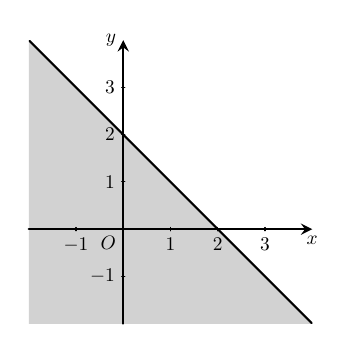
\begin{tikzpicture}[line join=round, line cap=round,>=stealth,thick,scale=0.6]
		\tikzset{every node/.style={scale=0.7}}
		\begin{scope}
		\clip (-2,-2) rectangle (4,4);
		\fill[black!35,opacity=0.5] (-3,5)--(-3,-3)--(5,-3)--cycle;
		\draw (-2,4)--(4,-2);% node [pos=0.45, above, sloped] {$x+y-2=0$};
		\end{scope}
		\draw[->] (-2,0)--(4,0) node[below]{$x$};
		\draw[->] (0,-2)--(0,4) node[left]{$y$};
		\draw (0,0) node[below left]{$O$};
		\foreach \x in {-1,1,2,3}
			\draw[thin] (\x,1pt)--(\x,-1pt) node [below] {$\x$};
		\foreach \y in {-1,1,2,3}
			\draw[thin] (1pt,\y)--(-1pt,\y) node [left] {$\y$};
		\end{tikzpicture}
	}
	{\True 
		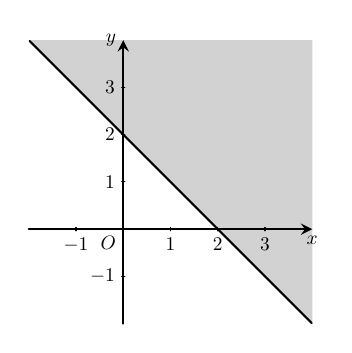
\begin{tikzpicture}[line join=round, line cap=round,>=stealth,thick,scale=0.6]
		\tikzset{every node/.style={scale=0.7}}
		\begin{scope}
		\clip (-2,-2) rectangle (4,4);
		\fill[black!35,opacity=0.5] (-3,5)--(5,5)--(5,-3)--cycle;
		\draw (-2,4)--(4,-2);% node [pos=0.45, above, sloped] {$x+y-2=0$};
		\end{scope}
		\draw[->] (-2,0)--(4,0) node[below]{$x$};
		\draw[->] (0,-2)--(0,4) node[left]{$y$};
		\draw (0,0) node[below left]{$O$};
		\foreach \x in {-1,1,2,3}
			\draw[thin] (\x,1pt)--(\x,-1pt) node [below] {$\x$};
		\foreach \y in {-1,1,2,3}
			\draw[thin] (1pt,\y)--(-1pt,\y) node [left] {$\y$};
		\end{tikzpicture}
	}
	{ 
		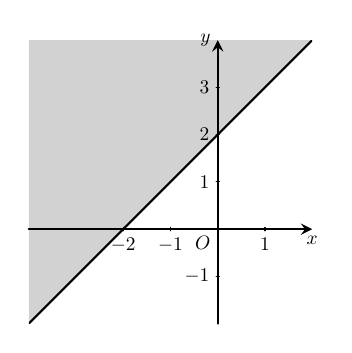
\begin{tikzpicture}[line join=round, line cap=round,>=stealth,thick,scale=0.6]
		\tikzset{every node/.style={scale=0.7}}
		\begin{scope}
		\clip (-4,-2) rectangle (2,4);
		\fill[black!35,opacity=0.5] (-5,-3)--(-5,5)--(3,5)--cycle;
		\draw (2,4)--(-4,-2);% node [pos=0.45, above, sloped] {$x-y+2=0$};
		\end{scope}
		\draw[->] (-4,0)--(2,0) node[below]{$x$};
		\draw[->] (0,-2)--(0,4) node[left]{$y$};
		\draw (0,0) node[below left]{$O$};
		\foreach \x in {-2,-1,1}
			\draw[thin] (\x,1pt)--(\x,-1pt) node [below] {$\x$};
		\foreach \y in {-1,1,2,3}
			\draw[thin] (1pt,\y)--(-1pt,\y) node [left] {$\y$};
		\end{tikzpicture}
	}
	{
		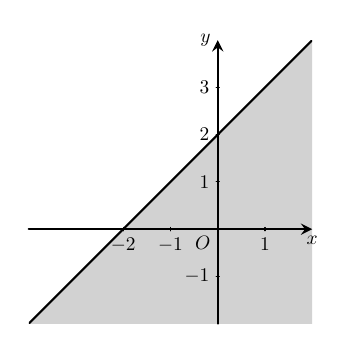
\begin{tikzpicture}[line join=round, line cap=round,>=stealth,thick,scale=0.6]
		\tikzset{every node/.style={scale=0.7}}
		\begin{scope}
		\clip (-4,-2) rectangle (2,4);
		\fill[black!35,opacity=0.5] (-5,-3)--(3,-3)--(3,5)--cycle;
		\draw (2,4)--(-4,-2);% node [pos=0.45, above, sloped] {$x-y+2=0$};
		\end{scope}
		\draw[->] (-4,0)--(2,0) node[below]{$x$};
		\draw[->] (0,-2)--(0,4) node[left]{$y$};
		\draw (0,0) node[below left]{$O$};
		\foreach \x in {-2,-1,1}
			\draw[thin] (\x,1pt)--(\x,-1pt) node [below] {$\x$};
		\foreach \y in {-1,1,2,3}
			\draw[thin] (1pt,\y)--(-1pt,\y) node [left] {$\y$};
		\end{tikzpicture}
	}
	\loigiai{
		Ta có $(d)\colon x+y=2$ đi qua $(0;2)$ và $(2;0)$.\\
		Mặt khác với $x=0$, $y=0$ thì $x+y=0<2$ nên miền nghiệm là nửa mặt phẳng có bờ là $(d)\colon x+y=2$ đi qua $(0;2)$, $(2;0)$ và chứa điểm $O(0;0)$ (kể cả bờ).
	}
\end{ex}
%Câu 11
\begin{ex}%[0H1Y2-1]%[Dự án đề kiểm tra HKI NH22-23-VU Ngoc Hao]%[VoNguyenGiap-QuangNam]
	Cho tam giác $ABC$ biết $BC=5$, $AC=3$, $AB=4$. Tính $\cos C$.
	\choice
	{$\cos C=-\dfrac{3}{5}$}
	{$\cos C=-\dfrac{4}{5}$}
	{$\cos C=-\dfrac{4}{5}$}
	{\True $\cos C=\dfrac{3}{5}$}
	\loigiai{
	Áp dụng định lí cô-sin trong tam giác $ABC$, ta có \[\cos C=\dfrac{CA^2 + CB^2 - AB^2}{2\cdot CA\cdot CB}=\dfrac{9+25-16}{2\cdot3\cdot5}=\dfrac{3}{5}.\]		}
\end{ex}
%Câu 12

\begin{ex}%[0H2Y2-2]%[Dự án đề kiểm tra HKI NH22-23-VU Ngoc Hao]%[VoNguyenGiap-QuangNam]
	Cho tam giác $ABC$, gọi $G$ là trọng tâm của tam giác $ABC$. Đẳng thức véc-tơ nào sau đây {\bf sai}?
	\choice
	{$\overrightarrow{GA}+\overrightarrow{GB}+\overrightarrow{GC}=\overrightarrow{0}$}
	{\True$\overrightarrow{GA}+\overrightarrow{GB}=-\overrightarrow{CG}$}
	{$\overrightarrow{GA}+\overrightarrow{GB}=\overrightarrow{CG}$}
	{$\overrightarrow{GA}+\overrightarrow{GB}=-\overrightarrow{GC}$}
	\loigiai{
	\immini{Ta có $\overrightarrow{GA}+\overrightarrow{GB}=-\overrightarrow{GC}$}
	{\begin{tikzpicture}[>=stealth,line join=round,line cap=round,font=\footnotesize,scale=1]
			\path 
			(0,0) coordinate (B)
			(4,0) coordinate (C)
			(1,2) coordinate (A)
			($(B)!0.5!(C)$) coordinate (M)
			($(A)!2/3!(M)$) coordinate (G)
			;
			\draw (A)--(B)--(C)--cycle (A)--(M);
			\foreach \l/\g in {A/90,B/180,C/-45,M/-90,G/0}
			\draw[fill=black] (\l) circle (1pt) +(\g:.3) node{$\l$};
	\end{tikzpicture}}

}
\end{ex}


%Câu 13
\begin{ex}%[0H2Y3-2]%[Dự án đề kiểm tra HKI NH22-23-VU Ngoc Hao]%[VoNguyenGiap-QuangNam]
	Cho tam giác $ABC$, gọi $M$ là trung điểm của $BC$ và $G$ là trọng tâm của tam giác $ABC$. Đẳng thức véc-tơ nào sau đây đúng?
	\choice
	{$\overrightarrow{MB} - \overrightarrow{MC} =\overrightarrow{0}$}
	{\True $2\overrightarrow{AM} = 3\overrightarrow{AG}$}
	{$3\overrightarrow{AM} = 2\overrightarrow{AG}$}
	{$\overrightarrow{BC} = 2\overrightarrow{CM}$}
	\loigiai{
		\immini{
			Vì $G$ là trọng tâm $\triangle ABC$ nên $AG = \dfrac{2}{3}AM \Rightarrow 2\overrightarrow{AG}=3\overrightarrow{AM}$.
		}{
			\begin{tikzpicture}[>=stealth,line join=round,line cap=round,font=\footnotesize,scale=1]
					\path 
						(0,0) coordinate (B)
						(4,0) coordinate (C)
						(1,2) coordinate (A)
						($(B)!0.5!(C)$) coordinate (M)
						($(A)!2/3!(M)$) coordinate (G)
					;
					\draw (A)--(B)--(C)--cycle (A)--(M);
					\foreach \l/\g in {A/90,B/180,C/-45,M/-90,G/0}
						\draw[fill=black] (\l) circle (1pt) +(\g:.3) node{$\l$};
			\end{tikzpicture}
		}
	}
\end{ex}

%Câu 14
\begin{ex}%[0D1Y1-1]%[Dự án đề kiểm tra HKI NH22-23-VU Ngoc Hao]%[VoNguyenGiap-QuangNam]
	Cho các phát biểu sau:
	\begin{enumEX}[1.]{1}
		\item \lq\lq 12 là số nguyên tố \rq\rq 
		\item \lq\lq Tam giác vuông có một đường trung tuyến bằng một nửa cạnh huyền\rq\rq 
		\item \lq\lq Các em hãy số gắng học tập thật tốt nhé\rq\rq 
		\item \lq\lq Học sinh trường THPT Võ Nguyên Giáp học giỏi Toán không?\rq\rq
	\end{enumEX}
	Hỏi có bao nhiêu phát biểu là mệnh đề?
	\choice
	{$3$}
	{$4$}
	{$1$}
	{\True $2$}
	\loigiai{
		Các phát biểu là mệnh đề là
		\begin{itemize}
			\item \lq\lq 12 là số nguyên tố \rq\rq 
			\item \lq\lq Tam giác vuông có một đường trung tuyến bằng một nửa cạnh huyền\rq\rq 
		\end{itemize}
	}
\end{ex}

%Câu 15
\begin{ex}%[0D1Y1-3]%[Dự án đề kiểm tra HKI NH22-23-VU Ngoc Hao]%[VoNguyenGiap-QuangNam]
	Cho số gần đúng $a=789\,246$ và độ chính xác $d=200$. Số quy tròn của số $a$ là
	\choice
	{$790\,000$}
	{$789\,200$}
	{\True $789\,000$}
	{$789\,240$}
	\loigiai{
		Số quy tròn của $a=789\,246$ với độ chính xác $d=200$ là $789\,000$.
	}
\end{ex}
  \begin{center}
  	\textbf{PHẦN 2 - TỰ LUẬN}
  \end{center}

%Bài 1
\begin{bt}%[0H1Y2-1]%[Dự án đề kiểm tra HKI NH22-23-VU Ngoc Hao]%[VoNguyenGiap-QuangNam]
	Cho $\triangle ABC$ biết $AC=b=3$ cm, $AB=c=6$ cm, $\widehat{A}=120^\circ$. Tính cạnh $BC$.
	\loigiai{
		Áp dụng định lý cô-sin ta có
		\[BC^2 = AB^2 + AC^2 - 2AB\cdot AC\cdot \cos A = 3^2 + 6^2 -2\cdot 3\cdot 6\cdot \cos 120^\circ = 63.\]
		Vậy $BC=\sqrt{63}=3\sqrt{7}$ cm.
	}
\end{bt}

%Bài 2
\begin{bt}%[0H3Y2-1]%[Dự án đề kiểm tra HKI NH22-23-VU Ngoc Hao]%[VoNguyenGiap-QuangNam]
	Trong mặt phẳng tọa độ $Oxy$, cho $2$ véc-tơ $\overrightarrow{a}=(4;2)$, $\overrightarrow{b}=(-3;6)$. Tính tích vô hướng $\overrightarrow{a}\cdot \overrightarrow{b}$ và chứng tỏ $\overrightarrow{a}\perp\overrightarrow{b}$.
	\loigiai{
		Ta có $\overrightarrow{a}\cdot \overrightarrow{b} = 4\cdot (-3) + 2\cdot 6 =0$.\\
		Suy ra $\overrightarrow{a}\perp\overrightarrow{b}$.
	}
\end{bt}

%Bài 3
\begin{bt}%[0D1Y3-4]%[Dự án đề kiểm tra HKI NH22-23-VU Ngoc Hao]%[VoNguyenGiap-QuangNam]
	Cho hai tập hợp $A=[1;+\infty)$, $B=(-3;2]$. Hãy tìm các tập hợp $A\cap B$, $C_{\mathbb{R}}\left(A\cap B\right)$.
	\loigiai{
		Ta có $A\cap B = [1;2]$.\\
		Suy ra $C_{\mathbb{R}}\left(A\cap B\right)=\mathbb{R}\setminus\left(A\cap B\right)=\left(-\infty;1\right)\cup \left(2;+\infty\right)$.
	}
\end{bt}

%Bài 4
\begin{bt}%[0H3K2-4]%[Dự án đề kiểm tra HKI NH22-23-VU Ngoc Hao]%[VoNguyenGiap-QuangNam]
	Trong hệ trục $Oxy$, cho hai điểm $A(-2;3)$, $B(-1;-3)$. Tìm điểm $D$ nằm trên đường thẳng $x+y=1$ sao cho $\triangle ABD$ vuông tại $D$.
	\loigiai{
		Vì $D\in (\Delta )\colon x+y=1$ nên $D\left(a;1-a\right)$.\\
		Khi đó $\overrightarrow{AD} = \left(a+2;-2-a\right)$, $\overrightarrow{BD}=(a+1;4-a)$.\\
		Ta có $\triangle ABD$ vuông tại $D$ khi và chỉ khi
		\allowdisplaybreaks
		\begin{eqnarray*}
		\overrightarrow{AD}\cdot \overrightarrow{BD} = 0
		&\Leftrightarrow& (a+2)(a+1) + (-2-a)(4-a)=0 \\
		&\Leftrightarrow&  a^2 +3a +2 -8 -4a +2a + a^2 =0\\
		&\Leftrightarrow& 2a^2 +a -6 = 0\\
		&\Leftrightarrow& \hoac{&a=-2\\&a=\dfrac{3}{2}.}
		\end{eqnarray*}
		Với $a=-2$ thì $D(-2;3)$ trùng với điểm $A(-2;3)$ nên loại.\\
		Với $a=\dfrac{3}{2}$ thì $D\left(\dfrac{3}{2};-\dfrac{1}{2}\right)$.\\
		Vậy điểm thỏa mãn yêu cầu là  $D\left(\dfrac{3}{2};-\dfrac{1}{2}\right)$.
		 
	}		
\end{bt}

%Bài 5
\begin{bt}%[0H2K3-5]%[Dự án đề kiểm tra HKI NH22-23-VU Ngoc Hao]%[VoNguyenGiap-QuangNam]
	Cho hình bình hành $ABCD$ tâm $O$. Gọi $E$ là trung điểm $AD$ và $G$ là trọng tâm tam giác $ABD$. Chứng minh rằng $\overrightarrow{GE} = \dfrac{1}{6}\overrightarrow{AD} - \dfrac{1}{3}\overrightarrow{AB}$.
	\loigiai{
		\immini
		{
			\allowdisplaybreaks
			\begin{eqnarray*}
				\overrightarrow{GE} =\overrightarrow{AE} - \overrightarrow{AG}
				&=& \dfrac{1}{2}\overrightarrow{AD} -\dfrac{2}{3}\overrightarrow{AO}\\
				&=& \dfrac{1}{2}\overrightarrow{AD} - \dfrac{2}{3}\cdot \dfrac{1}{2}\left(\overrightarrow{AB} + \overrightarrow{AD}\right)\\
				&=& \dfrac{1}{2}\overrightarrow{AD} - \dfrac{1}{3}\overrightarrow{AB} - \dfrac{1}{3}\overrightarrow{AD}\\
				&=& \dfrac{1}{6}\overrightarrow{AD} - \dfrac{1}{3}\overrightarrow{AB}.
			\end{eqnarray*}
		}
		{
			\begin{tikzpicture}[>=stealth,line join=round,line cap=round,font=\footnotesize,scale=1]
				\coordinate[label=below left:{$A$}] (A) at (0,0);
				\coordinate[label=above left:{$B$}] (B) at (1.5,2);
				\coordinate[label=above right:{$C$}] (C) at (5,2);
				\coordinate[label=below right:{$D$}] (D) at ($(A)+(C)-(B)$);
				\coordinate[label=below:{$O$}] (O) at (intersection of A--C and B--D);
				\coordinate[label=below:{$E$}] (E) at ($(A)!0.5!(D)$);
				\coordinate[label=below:{$G$}] (G) at ($(A)!2/3!(O)$);
				
				\draw (A)--(B)--(C)--(D)--cycle;
				\draw (A)--(C) (B)--(D);
				
				\foreach \p in {A,B,C,D,O,E,G}
				\fill (\p) circle (1.2pt);
			\end{tikzpicture}
		}
	}
\end{bt}

\Closesolutionfile{ans}
